\section{Motivation}

{ \setbeamercolor{background canvas}{bg=hl_bg}
  \setbeamercolor{normal text}{fg=hl_fg}
  \setbeamercolor{frametitle}{fg=hl_fg}
  \begin{frame}
    \usebeamercolor[fg]{normal text}
    \begin{center}
      {\large Why are Probabilistic Graphical Models interested?}
    \end{center}
  \end{frame}
}
\subsection{Directed}
\begin{frame}{Directed Graph Representation}
  \begin{itemize}
    
    \item 
      \begin{columns}
        \column{0.5\textwidth}
        \hskip 1cm
        \begin{tikzpicture}
          % \tikzstyle{enode} = [thick, draw=blue, circle, inner sep = 3pt,
          % align=center]
          \tikzstyle{enode} = [thick, draw=black, ellipse, inner sep = 2pt,  align=center]
          \tikzstyle{nnode} = [thick, rectangle, rounded corners = 2pt, minimum size = 0.5cm,draw,inner sep = 2pt]

          \node[enode] (s) at (-0.5, 1.5) {Sprinkler};
          \node[enode] (r) at (1.5, 1.5) {Rain};
          \node[enode] (gw) at (1, 0) {Grass Wet};
          \draw[->] (r) to (s);
          \draw[->] (r) to (gw);
          \draw[->] (s) to (gw);
        \end{tikzpicture}\\
        \centering
        Is the sprinkler working?
        
        \column{0.5\textwidth}
        \hskip -1cm
        \begin{tikzpicture}
          \tikzstyle{cnode} = [thick, draw=black, ellipse, inner sep = 1pt,  align=center]
          \tikzstyle{nnode} = [thick, rectangle, rounded corners = 0pt,draw,inner sep = 2pt]
          \node[cnode] (virus) at (0, 1.5) {Covid-19};
          \node[cnode] (fever) at (-3, 0) {Fever};
          \node[cnode] (cough) at (-1.5, 0) {Cough};
          \node[cnode] (breath) at (1, 0) {Breath Difficulty};
          \draw[->] (virus) -- (fever);
          \draw[->] (virus) -- (cough);
          \draw[->] (virus) -- (breath);
        \end{tikzpicture}\\
        \centering
        Is the person get contiguous by COVID?
      \end{columns}
    \item 
      \vskip 0.5cm
      \begin{columns}
        \column{0.5\textwidth}
        \hskip 1cm
        \begin{tikzpicture}[scale=0.8]
          \tikzstyle{enode} = [thick, draw, circle, inner sep = 3pt,  align=center]
          \tikzstyle{cnode} = [thick, fill=black, draw, circle, inner sep = 3pt,  align=center]
          \begin{scope}{scale=0.5, xshift=1cm}
            \node[enode] (x1) at (-2, 0) {};
            \node[enode] (x2) at (-1, 0) {};
            \node[enode] (x3) at (0, 0) {};
            \node[enode] (x4) at (1, 0) {};
            \node[text width=1cm, right = 0.2cm of x4] {Phoneme};
            \node[cnode] (y1) at (-2, -1.5) {};
            \node[cnode] (y2) at (-1, -1.5) {};
            \node[cnode] (y3) at (0, -1.5) {};
            \node[cnode] (y4) at (1, -1.5) {};
            \node[text width=1cm, right = 0.2cm of y4] {Acoustic};

            \draw[->] (x1) to (x2);
            \draw[->] (x2) to (x3);
            \draw[->] (x3) to (x4);

            \draw[->] (x1) to (y1);
            \draw[->] (x2) to (y2);
            \draw[->] (x3) to (y3);
            \draw[->] (x4) to (y4);

          \end{scope}
        \end{tikzpicture}
        \vskip 0.1cm
        \centering
        Speech Recognition
        \column{0.5\textwidth}
        \begin{tikzpicture}[scale=0.65]
          \tikzstyle{enode} = [thick, draw, circle, inner sep = 3pt,  align=center]
          \tikzstyle{cnode} = [thick, fill=gray, draw, circle, inner sep = 3pt,  align=center]
          \begin{scope}{scale=0.5, xshift=1cm}
            \node[cnode] (o1) at (-2, 1.5) {$\Oo_1$};
            \node[cnode] (o2) at (0, 1.5) {$\Oo_2$};
            \node[cnode] (o3) at (2, 1.5) {$\Oo_3$};
            \node[cnode] (o4) at (4, 1.5) {$\Oo_4$};
            \node[text width=1cm, right = 0.2cm of o4] {Award};

            \node[enode] (a1) at (-2, 0) {$a_1$};
            \node[enode] (a2) at (0, 0) {$a_2$};
            \node[enode] (a3) at (2, 0) {$a_3$};
            \node[enode] (a4) at (4, 0) {$a_4$};
            \node[text width=1cm, right = 0.2cm of a4] {Action};
            \node[enode] (s1) at (-2, -1.5) {$s_1$};
            \node[enode] (s2) at (0, -1.5) {$s_2$};
            \node[enode] (s3) at (2, -1.5) {$s_3$};
            \node[enode] (s4) at (4, -1.5) {$s_4$};
            \node[text width=1cm, right = 0.2cm of s4] {State};

            \draw[->] (s1) to (s2);
            \draw[->] (s2) to (s3);
            \draw[->] (s3) to (s4);
            \draw[->] (a1) to (s2);
            \draw[->] (a2) to (s3);
            \draw[->] (a3) to (s4);
            \draw[->] (s1) to [out=15, in=-15] (o1);
            \draw[->] (s2) to [out=15, in=-15] (o2);
            \draw[->] (s3) to [out=15, in=-15] (o3);
            \draw[->] (s4) to [out=15, in=-15] (o4);

          \end{scope}
          
        \end{tikzpicture}
        \centering
        Control, reinforcement learning        
      \end{columns}
    
  \end{itemize}

\end{frame}


\subsection{Directed}
\begin{frame}{Undirected Graph Representations}
  \begin{itemize}
  \item % image segmentation
        \begin{tikzpicture}
          \tikzstyle{enode} = [thick, draw, circle, inner sep = 3pt,  align=center]
          \tikzstyle{cnode} = [thick, fill=gray, draw, circle, inner sep = 3pt,  align=center]
          \begin{scope}{scale=0.4}
            \node[inner sep=0pt] (img) at (-7,0) {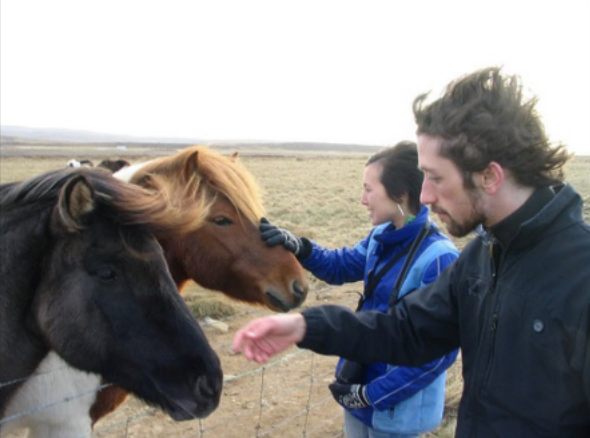
\includegraphics[width=.25\textwidth]{images/illustrate/slam_img.png}};
          \end{scope}
          \begin{scope}{scale=0.4}
            \node[inner sep=0pt] (slam) at (0,0) {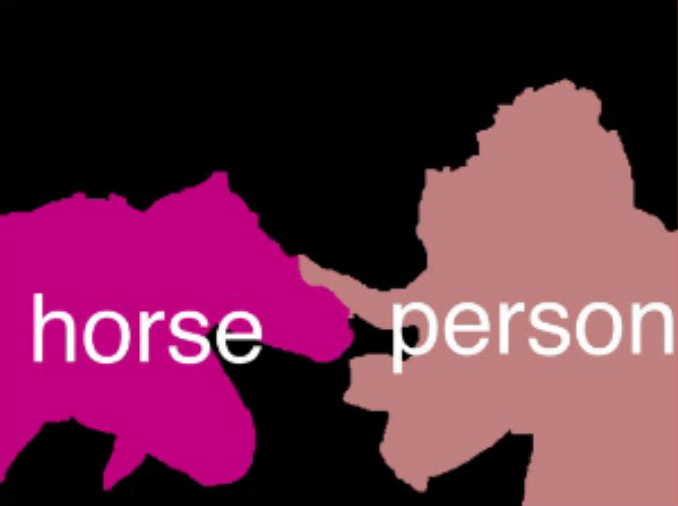
\includegraphics[width=.25\textwidth]{images/illustrate/slam_lab.png}};
          \end{scope}
          
          \begin{scope}[local bounding box=crf, scale=0.6, xshift=-4cm]
            \node[enode] (x1) at (-2, 1) {};
            \node[enode] (x2) at (0, 1) {};
            \node[enode] (x3) at (-2, -1) {};
            \node[enode] (x4) at (0, -1) {};

            \node[cnode] (y1) at (-3, 0) {};
            \node[cnode] (y2) at (-1, 0) {};
            \node[cnode] (y3) at (-3, -2) {};
            \node[cnode] (y4) at (-1, -2) {};
            \node[text width=1cm, left = 0.2cm of x1] {Label};
            \node[text width=1cm, right = 0.2cm of y4] {Pixel};

            \draw[-] (x1) to (y1);
            \draw[-] (x2) to (y2);
            \draw[-] (x3) to (y3);
            \draw[-] (x4) to (y4);

            \draw[-] (x1) to (x2);
            \draw[-] (x1) to (x3);
            \draw[-] (x2) to (x4);
            \draw[-] (x3) to (x4);
          \end{scope}
          
        \end{tikzpicture}
        \vskip 0.1cm
        \centering
        Vision Perception
        \item % digital communication
        \begin{tikzpicture}[scale=0.7]
          \tikzstyle{enode} = [thick, draw, circle, inner sep = 3pt,  align=center]
          \tikzstyle{cnode} = [thick, fill=gray, draw, circle, inner sep = 3pt,  align=center]
      
          \begin{scope}[local bounding box=mrf]{scale=0.2}
            \node[enode] (x1) at (-2, 1) {};
            \node[enode] (x2) at (-1, 1) {};
            \node[enode] (x3) at (0, 1) {};

            \node[cnode] (y1) at (-3, -1) {};
            \node[cnode] (y2) at (-1, -1) {};
            \node[cnode] (y3) at (1, -1) {};
            
            \node[text width=1cm, right = 0.2cm of x3] {True Symbol};
            \node[text width=1cm, right = 0.2cm of y3] {Received Symbol};

            \draw[-] (x1) to (y1);
            \draw[-] (x1) to (y2);
            \draw[-] (x1) to (y3);

            \draw[-] (x2) to (y1);
            \draw[-] (x2) to (y2);
            \draw[-] (x2) to (y3);

            \draw[-] (x3) to (y1);
            \draw[-] (x3) to (y2);
            \draw[-] (x3) to (y3);

          \end{scope}

          \begin{scope}[shift={(-4,0)}, scale=0.9, every node/.append style={transform shape}]
          \node[block](tx) at (-6,-1) {transmitter};
          \node[antenna] at (tx.east) {};
          \node[block,right = 1.5cm of tx](rx){receiver};
          \node[antenna,xscale=-1] at (rx.west) {};
          \end{scope}
        \end{tikzpicture}
        \centering
        Digital communication
      \item % Solid physics
        \begin{columns}
          \column{0.5\textwidth}
          \centering
        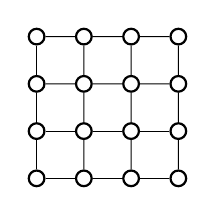
\begin{tikzpicture}
          \tikzstyle{enode} = [thick, draw, circle, inner sep = 2pt,  align=center]
          \tikzstyle{cnode} = [thick, fill=gray, draw, circle, inner sep = 3pt,  align=center]
      
          \begin{scope}[local bounding box=mrf, scale=0.6]
            \node[enode] (x11) at (0, 0) {};
            \node[enode] (x12) at (1, 0) {};
            \node[enode] (x13) at (2, 0) {};
            \node[enode] (x14) at (3, 0) {};
            \node[enode] (x21) at (0, 1) {};
            \node[enode] (x22) at (1, 1) {};
            \node[enode] (x23) at (2, 1) {};
            \node[enode] (x24) at (3, 1) {};
            \node[enode] (x31) at (0, 2) {};
            \node[enode] (x32) at (1, 2) {};
            \node[enode] (x33) at (2, 2) {};
            \node[enode] (x34) at (3, 2) {};
            \node[enode] (x41) at (0, 3) {};
            \node[enode] (x42) at (1, 3) {};
            \node[enode] (x43) at (2, 3) {};
            \node[enode] (x44) at (3, 3) {};

            \draw (x11)--(x12)--(x13)--(x14);
            \draw (x21)--(x22)--(x23)--(x24);
            \draw (x31)--(x32)--(x33)--(x34);
            \draw (x41)--(x42)--(x43)--(x44);

            \draw (x11)--(x21)--(x31)--(x41);
            \draw (x12)--(x22)--(x32)--(x42);
            \draw (x13)--(x23)--(x33)--(x43);
            \draw (x14)--(x24)--(x34)--(x44);
          \end{scope}
        \end{tikzpicture}\\
        \centering
        Physics (Ising or Potts model)
        \column{0.5\textwidth}
        \begin{itemize}[label=$\bullet$]
        \item Error-control codes
        \item Computational biology
        \item Natural language processing
        \item etc.
        \end{itemize}
      \end{columns}
  \end{itemize}


\end{frame}


%%% Local Variables:
%%% mode: latex
%%% TeX-master: "../ppgm_slide"
%%% End:
